\documentclass{article}
\usepackage[headheight=40pt, textheight=560pt]{geometry}
\usepackage{paralist}
\usepackage{scalerel,amssymb}
\usepackage{amsmath}
\usepackage{colortbl}
\usepackage{array}
\usepackage{multirow}
\usepackage{blindtext}
\usepackage{reledmac}
\usepackage{changepage}

\usepackage{pgfplots}
\usepackage{tikz}
\usetikzlibrary{positioning}
\usetikzlibrary{shapes.geometric, arrows}
\tikzstyle{arrow} = [thick,->,>=stealth]

\usepackage{graphicx}
\usepackage{stix}

\newcommand{\tableflip}{$($\rotatebox{45}{$\smile$}$^{\circ}\smwhtsquare^{\circ})\rotatebox{45}{$\smile$}\mkern-6mu\frown$\raisebox{0.5ex}{$\bot$}$\mkern-3.5mu-\mkern-3.5mu$\raisebox{0.5ex}{$\bot$}}

\usepackage{stackengine}
\def\apeqA{\SavedStyle\sim}
\def\apeq{\setstackgap{L}{\dimexpr.5pt+1.5\LMpt}\ensurestackMath{%
  \ThisStyle{\mathrel{\Centerstack{{\apeqA} {\apeqA} {\apeqA}}}}}}

\usepackage{fancyhdr}
\fancyhead[L]{
	\begin{tabular}{lll}
		\begin{tabular}{l}
			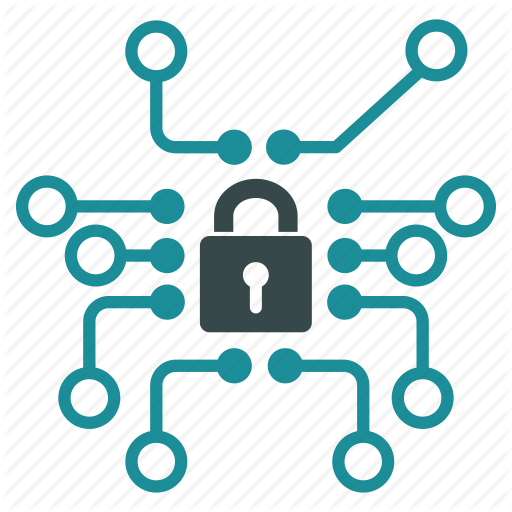
\includegraphics[scale=0.07]{security_lock}
		\end{tabular}	
		&
		\begin{tabular}{l}
			\LARGE \textbf{Cryptography} \\
			\Large \textsc{Zusammenfassung}
		\end{tabular}
		&
		\begin{tabular}{l}
			\tableflip
		\end{tabular}
	\end{tabular}
}
\fancyhead[R]{16-124-836 \\
Marcel \textsc{Zauder}}
\renewcommand{\headrulewidth}{0.4pt}
\fancyfoot[C]{\thepage}
\renewcommand{\footrulewidth}{0.4pt}

\usepackage{hyperref}

\begin{document}
	\pagestyle{fancy}
	\section{One Time Pad}
		\begin{adjustwidth}{2em}{}
			\subsection{What is [\textsc{not}] \textsc{Cryptography}}
			\begin{adjustwidth}{2em}{}
				\subsubsection{Introduction}
					\begin{adjustwidth}{2em}{4em}
						In the idealized model we assume that Alice wants to send a message $m$ (\textit{privately}) to Bob. Alice will modify the message $m$, also called \textit{\textbf{plaintext}}, with any method to create a \textit{\textbf{ciphertext}} $c$ which will be actually sent to Bob. This transformation is also called encryption (\textit{\textbf{Enc}}). After receiving the ciphertext $c$, Bob will reverse the step of transforming by using a decription algorithm (\textit{\textbf{Dec}}) to (\textit{hopefully}) get the original plaintext $m$. \\
						\textit{\textbf{\textsc{Note:}}} We are not trying to hide that a message is sent, so an \textbf{\textsc{Eavesdropper}} (an attacker between Alice and Bob) can obtain the ciphertext $c$ at any instance. Hiding the existence of communication is called \textit{steganography}.
						\\
						\begin{adjustwidth}{1em}{}
							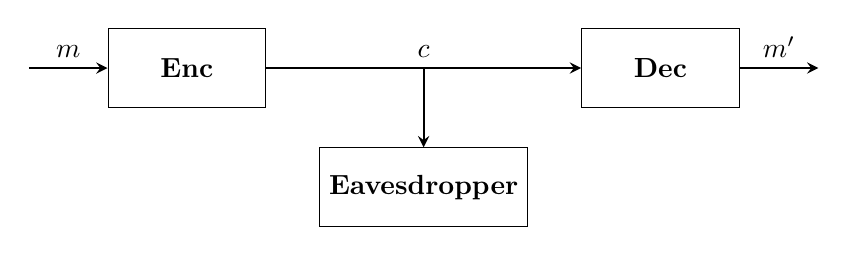
\begin{tikzpicture}
								\coordinate (start);
							
								%Nodes
								\node (rect) [draw,thin,minimum width=2cm,minimum height=1cm, right=of start] (Enc) {\textsc{\textbf{Enc}}};
								\node (rect) [draw,thin,minimum width=2cm,minimum height=1cm, right=4cm of Enc] (Dec) {\textsc{\textbf{Dec}}};
								\node (rect) [draw,thin,minimum width=2cm,minimum height=1cm, below right=0.5cm and 0.675cm of Enc] (Eve) {\textsc{\textbf{Eavesdropper}}};
								\node [right=of Dec] (stop) {};
							
								%Lines
								\draw[arrow] (start) -- node[ anchor=south ]{$m$} (Enc.west);
								\draw[arrow] (Enc.east) -- node[ anchor=south ]{$c$} (Dec.west);
								\draw[arrow] (Enc.east) -| (Eve.north);
								\draw[arrow] (Dec.east) -- node[ anchor=south ]{$m'$} (stop.west);
							
							\end{tikzpicture}
						\end{adjustwidth}
					\end{adjustwidth}
				\subsubsection{Kerckhoff's principle}
				\begin{adjustwidth}{2em}{4em}
					\textit{The method must not be required to be secret, and it must be able to fall into the enemy's hands without causing any inconvenience.} \\ \\
					So if the algorithm do not need to be secret, there must be additional information in the system, which is kept secret from any \textsc{\textbf{Eavesdropper}}. This information is called a \textbf{(secret) key} $k$. 
					\\
					\begin{adjustwidth}{1em}{}
						\begin{tikzpicture}							
							%Nodes
							\node (rect) [draw,thin,minimum width=2cm,minimum height=1cm, right=of start] (KeyGen) {\textsc{\textbf{KeyGen()}}};
							\node [below=of KeyGen] (start) {};
							\node (rect) [draw,thin,minimum width=2cm,minimum height=1cm, right=of start] (Enc) {\textsc{\textbf{Enc}}};
							\node (rect) [draw,thin,minimum width=2cm,minimum height=1cm, below right=0.5cm and 0.675cm of Enc] (Eve) {\textsc{\textbf{Eavesdropper}}};
							\node (rect) [draw,thin,minimum width=2cm,minimum height=1cm, right=4cm of Enc] (Dec) {\textsc{\textbf{Dec}}};
							\node [right=of Dec] (stop) {};
							
							%Lines
							\draw[arrow] (KeyGen.east) -| node[ anchor=south ]{$k$} (Enc.north);
							\draw[arrow] (KeyGen.east) -| node[ anchor=south ]{$k$} (Dec.north);
							\draw[arrow] (start) -- node[ anchor=south ]{$m$} (Enc.west);
							\draw[arrow] (Enc.east) -- node[ anchor=south ]{$c$} (Dec.west);
							\draw[arrow] (Enc.east) -| (Eve.north);
							\draw[arrow] (Dec.east) -- node[ anchor=south ]{$m'$} (stop.west);
							
						\end{tikzpicture}
					\end{adjustwidth}
				\end{adjustwidth}
			\end{adjustwidth}
		\end{adjustwidth}
		\newpage
		\begin{adjustwidth}{2em}{}
			\subsection{Specifics of \textsc{One-Time Pad}}
			\begin{adjustwidth}{2em}{4em}
				A \textit{one-time pad} often uses a secret key in the form of a bit string of length $\lambda$. The plain- and ciphertexts are also $\lambda$bit-strings. \\
				The construction of such an one-time pad looks as follows:
				\\
				\begin{adjustwidth}{2em}{}
					\begin{tabular}{lllll}
						\begin{tabular}{|l|}
							\hline
							\underline{\textsc{KeyGen()}} \\
							\ $k \leftarrow \{ 0,1 \} ^{\lambda}$ \\
							\ \textbf{return} $k$ \\
							\hline
						\end{tabular}
						&
						&
						\begin{tabular}{|l|}
							\hline
							\underline{\textsc{Enc}($k$, $m \in \{ 0,1 \} ^{\lambda}$)} \\
							\ $c := k \oplus m$ \\
							\ \textbf{return} $c$ \\
							\hline
						\end{tabular}
						&
						&
						\begin{tabular}{|l|}
							\hline
							\underline{\textsc{Dec}($k$, $c \in \{ 0,1 \} ^{\lambda}$)} \\
							\ $m' := k \oplus c$ \\
							\ \textbf{return} $m'$ \\
							\hline
						\end{tabular}
					\end{tabular}
				\end{adjustwidth}
				\hfill \\
				Recapture that $k \leftarrow \{ 0,1 \} ^{\lambda}$ means that $k$ is sampled uniformly from the set of $\lambda$bit-strings. \\
				Further we claim that for all $k,m \in \{ 0,1 \} ^{\lambda}$ it is true, that $Dec(k,Enc(k,m)) = m$. \\
				Otherwise the usage of one-time pad would be silly. \\
				For security reasons we want to say about the encryption scheme that an \textsc{Eavesdropper} (who does not know $k$) cannot leran anything about the message $m$. \\
				In the end we need to claim that an encryption algorithm is secure if for every $m \in \{ 0,1 \} ^{\lambda}$ the distribution \textsc{Eavesdrop}($m$) is the \textbf{uniform distribution} of $\{ 0,1 \} ^{\lambda}$, explicitly for every $m,m' \in \{ 0,1 \} ^{\lambda}$ the distributions \textsc{Eavesdrop}($m$) and \textsc{Eavesdrop}($m'$) are identical.
			\end{adjustwidth}
		\end{adjustwidth}
		
	\section{The Basics of Proveable Security}
		\begin{adjustwidth}{2em}{}
			\subsection{Generalizing and Abstracting One-Time Pad}
			\begin{adjustwidth}{2em}{}
				\subsubsection{Syntax \& Correctness}
				\begin{adjustwidth}{2em}{4em}
					A \textbf{symmetric key encryption \textit{(SKE)} scheme} consissts of the following algorithms:
					\begin{enumerate}[$\triangleright$]
						\item \textsc{KeyGen}: a randomized algorithm that outputs a \textbf{\textit{key}} $k \in K$
						\item \textsc{Enc}: a (\textit{possibly randomized}) algorithm that takes a key $k \in K$ and \textbf{\textit{plaintext}} $m \in M$ as input, and ouputs a \textbf{\textit{ciphertext}} $c \in C$
						\item \textsc{Dec}: a deterministic algorithm that takes a key $k \in K$ and a ciphertexts $c \in C$ as input, and outputs a plaintext $m \in M$
					\end{enumerate}
					$K$ is called the \textbf{\textit{key space}}, $M$ the \textbf{\textit{message space}}, and $C$ the \textbf{\textit{ciphertext space}} of the scheme. Often the entire scheme (with all its algorithms) is referred to as $\Sigma$. Each component is then referred to as $\Sigma$.\textsc{KeyGen}, $\Sigma$.\textsc{Enc}, $\Sigma$.\textsc{Dec}, $\Sigma.K$, $\Sigma.M$, and $\Sigma.C$. \\ \\
					Furthermore we define an encryption scheme to be \textbf{\textit{correct}} if for all $k \in K$ and all $m \in M$:
					\[
						Pr[\Sigma.\textsc{Dec}(k, \Sigma.\textsc{Enc}(k, m))=m] \ = \ 1 
					\]
					In other words, decrypting a ciphertext, using the same key used for encryption, \textbf{\textit{always}} results in the original plaintext.
				\end{adjustwidth}
			\end{adjustwidth}
			\newpage
			\subsection{Towards an Abstract Security Definition}
			\begin{adjustwidth}{2em}{4em}
				With the properties of one-time pad shown in the first chapter a first attempt can be made to define security: \\
				\textit{For all $m \in \{ 0,1 \}^{\lambda}$, the output of the following subroutine is uniformly distributed over $\{ 0,1 \}^{\lambda}$:}
				\begin{center}
					\begin{tabular}{|l|}
						\hline
						\underline{\textsc{Eavesdrop}($m \in \{ 0,1 \}^{\lambda}$):} \\
						\ \ $k \leftarrow \{ 0,1 \}^{\lambda}$ \\
						\ \ $c \ := \ k \oplus m$ \\
						\ \ \textbf{return} $c$ \\
						\hline
					\end{tabular}
				\end{center}
				\hfill \\
				This property is too specific to one-time pad. To get a more general-purpose security definition, we can write the subroutine using the totally generic encryption scheme $\Sigma$: \\
				\begin{center}
					\begin{tabular}{|l|}
						\hline
						\underline{\textsc{Eavesdrop}($m \in \Sigma.M$):} \\
						\ \ $k \leftarrow \Sigma.K$ \\
						\ \ $c \ := \ \Sigma.\textsc{Enc}(k,m)$ \\
						\ \ \textbf{return} $c$ \\
						\hline
					\end{tabular}
				\end{center}
				\hfill \\
				Such an encryption scheme $\Sigma$ is secure if, for all $m \in \Sigma.M$, the output of this subroutine is uniformly distributed over $\Sigma.C$. 
				\subsubsection{Adversary as Distinguishers}
				\begin{adjustwidth}{2em}{}
				Filler
				\end{adjustwidth}
				\subsubsection{Critically Analyzing a Security Definition}
				\begin{adjustwidth}{2em}{}
				Filler
				\end{adjustwidth}
				\subsubsection{Chosen Plaintext Attack Template}
				\begin{adjustwidth}{2em}{}
				Filler
				\end{adjustwidth}
			\end{adjustwidth}
			\subsection{Provable Security Fundamentals}
			\begin{adjustwidth}{2em}{}
				\subsubsection{Libraries \& Interfaces}
				\begin{adjustwidth}{2em}{}
				Filler
				\end{adjustwidth}
				\subsubsection{Semantics \& Scopes}
				\begin{adjustwidth}{2em}{}
				Filler
				\end{adjustwidth}
				\subsubsection{Interchangeability}
				\begin{adjustwidth}{2em}{}
				Filler
				\end{adjustwidth}
				\subsubsection{Security Definition, Using New Terminology}
				\begin{adjustwidth}{2em}{}
				Filler
				\end{adjustwidth}
			\end{adjustwidth}
			\subsection{How to Prove Security with the Hybrid Technique}
			\begin{adjustwidth}{2em}{}
				\subsubsection{Chaining Several Components}
				\begin{adjustwidth}{2em}{}
				Filler
				\end{adjustwidth}
				\subsubsection{One-Time Secrecy of One-Time Pad}
				\begin{adjustwidth}{2em}{}
				Filler
				\end{adjustwidth}
			\end{adjustwidth}
			\subsection{How to Demonstarte Insecurity with Attacks}
			\begin{adjustwidth}{2em}{}
			Filler
			\end{adjustwidth}
		\end{adjustwidth}
	
\end{document}